\section{Тюнинг SVM классификатора}
Изучим влияние значения параметра {\it Cost} штрафной функции SVM классификатора на
качество модели.
Результаты, представленные в таблицах \ref{table:results2015} и \ref{table:results2016},
были получены при значении по-умолчанию, $Cost=1$.

\begin{figure}[!htp] \centering
    \captionsetup[subfigure]{justification=centering}
    \begin{subfigure}[b]{0.45\textwidth}
        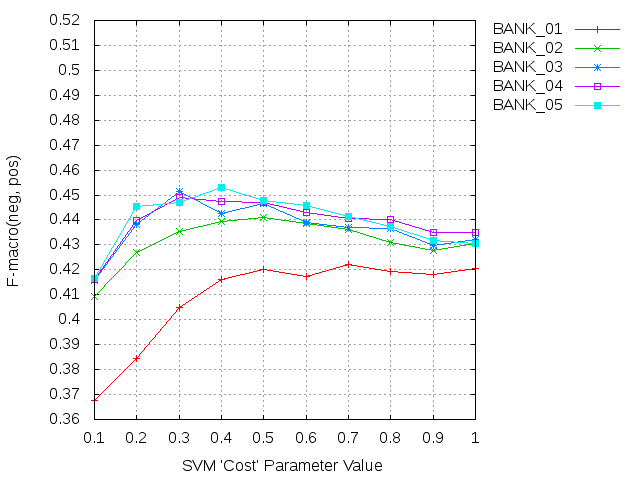
\includegraphics[width=\textwidth]{pics/2015_bank_balanced.png}
        \caption{BANK}
        \label{fig:bank_cost_changes_2015}
    \end{subfigure}
    ~
    \begin{subfigure}[b]{0.45\textwidth}
        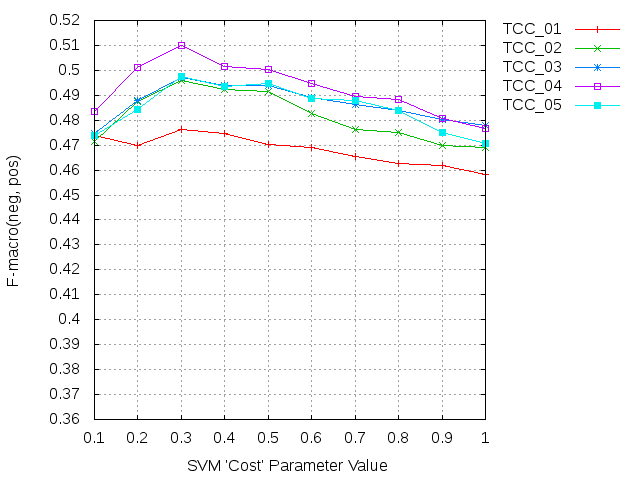
\includegraphics[width=\textwidth]{pics/2015_ttk_balanced.png}
        \caption{TCC}
        \label{fig:ttk_cost_changes_2015}
    \end{subfigure}

    \begin{subfigure}[b]{0.45\textwidth}
        \includegraphics[width=\textwidth]{pics/2016_ttk_balanced.png}
        \caption{TCC}
        \label{fig:ttk_cost_changes_2016}
    \end{subfigure}

    \caption{
        Влияние {\it параметра штрафной функции SVM классификатора}
        на результаты прогонов;
        кривыми на графиках обозначается прогоны с соответсвующими номерами;
        значение параметра измерялось в пределе $[0.1, 1]$ с шагом $0.1$.
    }
    \label{fig:cost}
\end{figure}
